\documentclass[reqno,12pt,onecolumn]{report}
% right side numbers for equations
% text size is 12 pt
% document has one column
% use TeXstudio to build this file

%SINCE THIS USES BIBER FOLLOW THE STEPS BELOW
%Option>Configure TeXstudio>Build>Default Bibliographic Tool: Biber
%IF YOU ADD NEW CITATIONS:
% F6: Compile
% F8: Bibtex (Biber)
% F5: Build and View

%FOR LIST OF SYMBOLS:
%Option>Configure TeXstudio>Commands>Makeindex then APPEND: %.nlo -s nomencl.ist -o %.nls

%IF YOU ADD NEW NOMENCLATURE ITEMS:
% Update the List of Symbols by clicking on Tools>Index
% F6: Compile
% F5: Build and View
%DO NOT MODIFY THIS FILE
\renewcommand{\rmdefault}{phv} % Arial
\renewcommand{\sfdefault}{phv} % Arial
% set font to Arial
\usepackage[top=1in,bottom=1in,left=1.5in,right=1in]{geometry}
% set the margins
\usepackage{amsmath,amsxtra,amsthm,amssymb,amsfonts}
% various AMS packages
\usepackage{graphicx,rotating,epsfig,epstopdf}
% insert and rotate images
%\usepackage[subfigure]{tocloft}
\usepackage{tocloft}
% modify toc, lot, lof
\usepackage{afterpage,subcaption}
% subfigures in a figure: subfigure can replace subcaption
\usepackage{setspace}
% allows you to specify the line spacing
\doublespacing 
\usepackage{hyphenat}
%[none] no hyphenation
%\usepackage{fixltx2e}
% text superscript or subscript
\usepackage{multirow,titlesec}
% tables with multiple rows and edit chapter format
\usepackage{indentfirst,mdwlist,array}
% always indent the first paragraph
% compact version of list environments
\usepackage{algorithm,algorithmicx,algpseudocode}
% insert pseudo-codes in the document
\usepackage{morefloats,easylist,paralist,enumitem,rotfloat}
% increase the maximum number of figures
% nested list with a depth > 4
% inline list
\usepackage{url,hyperref,gloss}
% url: for bibliography with type misc, howpublished=\url{}
% hyperref: autoref of numbered items and bibliography field: url = 
% gloss: create a glossary
\usepackage[usenames,dvipsnames,svgnames,table]{xcolor}
%use colors for texts and tables
\usepackage{pgfgantt,tikz}%,pgf}
% pgfgantt: produce Ghantt charts
% tikz: graphics using commands (w/pgf)
% pgf: 
\usepackage{longtable}
%==========================================================
\renewcommand{\contentsname}{\hfill Table of Contents\hfill}
% change the title of toc
\renewcommand{\cfttoctitlefont}{\normalfont\bfseries}
\renewcommand{\cftaftertoctitle}{\hfill}
% centered and bold header for toc
\usepackage{titletoc}
% title of toc
\titlecontents*{chapter}% <section-type>
[0pt]% <left>
{}% <above-code>
{\bfseries\chaptername\ \thecontentslabel \quad}% <numbered-entry-format>
{\bfseries\ \thecontentslabel }% <numberless-entry-format>
{\bfseries \hfill \contentspage \\}% <filler-page-format>
% add Chapter to each chapter in toc and no dots
\titlecontents*{section}
[0pt]
{}
{\hspace{65pt} \thecontentslabel \quad}
%{\quad \quad \quad \quad \thecontentslabel \quad}
{}
{\hfill \contentspage \\}
% remove dots
\titlecontents*{subsection}
[0pt]
{}
{\hspace{95pt} \thecontentslabel \quad}
%{\quad \quad \quad \quad \thecontentslabel \quad}
{}
{\hfill \contentspage \\}
% remove dots

\titlespacing*{\chapter}{0pt}{0pt}{12pt}
%\titlespacing*{command}{left}{before-sep}{after-sep}[right-sep]

\titleformat{\chapter}[display]{\normalfont \normalfont \bfseries \centering }{\chaptertitlename\ \thechapter}{8pt}{\normalfont \bfseries \centering}
% control the output of \chapter{}
\titleformat{\section}{\normalfont\bfseries}{\thesection}{1em}{}
% control the output of \section{}
\titleformat{\subsection}{\normalfont\bfseries}{\thesubsection}{1em}{}
% control the output of \subsection{}
\renewcommand{\cftlottitlefont}{\hfill\normalfont\bfseries}
\renewcommand{\cftafterlottitle}{\hfill}
% change the title of lot
\renewcommand{\cftloftitlefont}{\hfill\normalfont\bfseries}
\renewcommand{\cftafterloftitle}{\hfill}
% change the title of lof
\usepackage[final]{pdfpages}
%==========================================================
\usepackage[toc]{appendix}
% appendices in the thesis
%==========================================================
\usepackage[backend=biber,bibstyle=ieee,sorting=rmc,defernumbers=true]{biblatex}
\DeclareSortingScheme{rmc}{
\sort{
\field{keywords} 
}
}
%==========================================================
\usepackage{nomencl}
\makenomenclature
%END OF PREAMBLE

%==========================================================
%-----> REFERENCE DATABASE FROM THE GROUP MEMBERS
%-----> REQUIRED FOR PROPOSAL
%-----> TO BE UPDATED DURING PROJECT 1 AND PROJECT 2
\addbibresource{GroupName_Member1.bib} 
\addbibresource{GroupName_Member2.bib} 
%==========================================================
\begin{document}
\pagenumbering{roman}
%-----> FILE CONTAINING THE COVER PAGE
\input{GroupName_Cover} 
\newpage
%-----> FILE CONTAINING THE APPROVAL SHEET
%-----> REQUIRED IN PROJECT 2
\input{GroupName_ApprovalSheet_2023_02_20} 
\addtocontents{toc}{~\hfill\textbf{Page}}
%==========================================================
\newpage
\addcontentsline{toc}{chapter}{Abstract}
\chapter*{Abstract}
%-----> FILE CONTAINING THE ABSTRACT
%-----> REQUIRED IN PROJECT 2
\input{GroupName_Abstract} 
%==========================================================
\newpage
\addcontentsline{toc}{chapter}{Acknowledgment}
\chapter*{Acknowledgment}
%-----> FILE(S) CONTAINING THE ACKNOWLEDGEMNT 
%-----> REQUIRED IN PROJECT 2
\input{GroupName_Acknowledgment} 
%==========================================================
%COMMANDS FOR TABLE OF CONTENTS
\newpage
\tableofcontents
%==========================================================
%COMMANDS FOR LIST OF TABLES
\newpage
\addcontentsline{toc}{chapter}{\protect List of Tables}
{
\addtocontents{lot}{~\hfill\textbf{Page}\par}
\renewcommand{\cftdot}{ }
\makeatletter
\listoftables
}
%==========================================================
%COMMANDS FOR LIST OF FIGURES
\newpage
\addcontentsline{toc}{chapter}{\protect List of Figures}
{
\addtocontents{lof}{~\hfill\textbf{Page}\par}
\renewcommand{\cftdot}{ }
\makeatletter
\listoffigures
}
%==========================================================
%COMMANDS FOR LIST OF SYMBOLS
\newpage
\addcontentsline{toc}{chapter}{\protect List of Figures}
{
\addtocontents{los}{~\hfill\textbf{Page}\par}
\renewcommand{\cftdot}{ }
\makeatletter
\renewcommand{\nomname}{List of Symbols}
\printnomenclature 
}
%==========================================================
%START OF ARABIC PAGINATION
\newpage
\pagenumbering{arabic}
%==========================================================
\chapter{INTRODUCTION}
\label{chap:intro}
%-----> FILE(S) FOR THE INTRODUCTION
%-----> REQUIRED FOR PROPOSAL
%-----> MUST BE UPDATED IN PROJECT 1 and 2
\input{GroupName_Introduction} 
%==========================================================
\chapter{THEORETICAL BACKGROUND}
\label{chap:theoretical}
%-----> FILE(S) FOR THE THEORETICAL BACKGROUND
%-----> REQUIRED FOR PROPOSAL
%-----> MUST BE UPDATED IN PROJECT 1 and 2
\input{GroupName_Theoretical} 
%==========================================================
\chapter{RESEARCH METHODOLOGY}
\label{chap:method}
%-----> FILE(S) FOR THE METHODOLOGY
%-----> REQUIRED FOR PROPOSAL
%-----> MUST BE UPDATED IN PROJECT 1 and 2
\input{GroupName_Methodology} 
%==========================================================
\chapter{RESULTS AND DISCUSSIONS}
\label{chap:results}
%-----> FILE(S) FOR THE RESULTS AND DISCUSSIONS
%-----> REQUIRED IN PROJECT 1
%-----> MUST BE UPDATED IN PROJECT 2
\input{GroupName_Results}  
%==========================================================
\chapter{CONCLUSIONS AND RECOMMENDATIONS}
\label{chap:conclusion}
%-----> FILE(S) FOR THE CONCLUSIONS AND RECOMMENDATIONS
%-----> REQUIRED IN PROJECT 2
\input{GroupName_Conclusions}  
%==========================================================
\newpage
\addcontentsline{toc}{chapter}{BIBLIOGRAPHY}
%-----> keywords should be included as one of the fields in the bib file
%-----> the bib files are loaded using \addbibresource in the preamble
\chapter*{BIBLIOGRAPHY}
\printbibliography[keyword=Books, heading=subbibliography,title={Books}]
\printbibliography[keyword=Published, heading=subbibliography,title={Published}]
\printbibliography[keyword=Unpublished, heading=subbibliography,title={Unpublished}]
\printbibliography[keyword=Electronic Sources, heading=subbibliography,title={Electronic Sources}]
%==========================================================
\newpage
\appendix
\renewcommand{\chaptername}{\appendixname}
\addtocontents{toc}{\protect\renewcommand\protect\chaptername{\appendixname}}
\chapter{PRIOR ART SEARCH and ANALYSIS REPORT}
%-----> REQUIRED FOR PROPOSAL
%-----> MUST BE UPDATED IN PROJECT 1 and 2
%Based on your output in the Workshop on Patent Search, print the docx file to pdf then insert it here.
%Each member should have an output for each pdf file below. 
%Use the official template from ITSO
%use includegraphics for the 1st page of the 1st document only
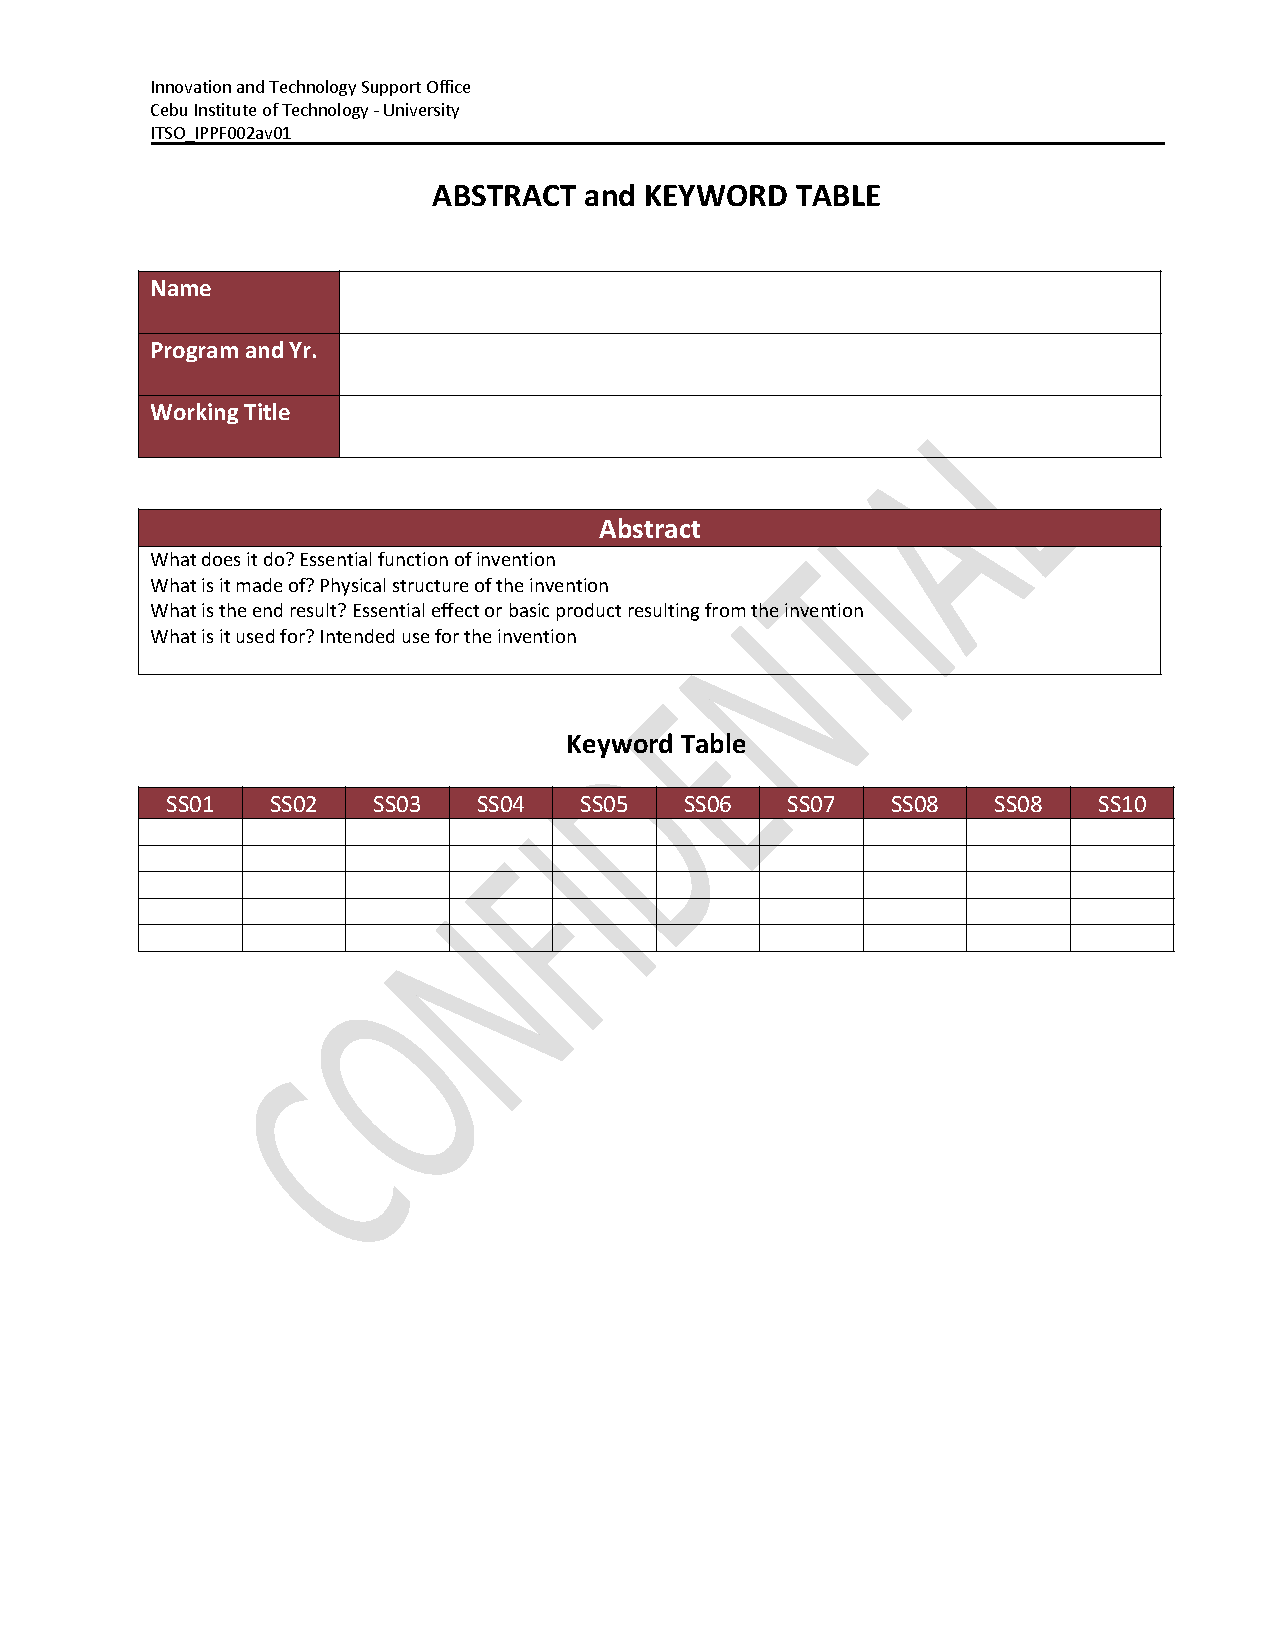
\includegraphics[page=1,width=\textwidth]{App_AbstractKeyword_member1.pdf}
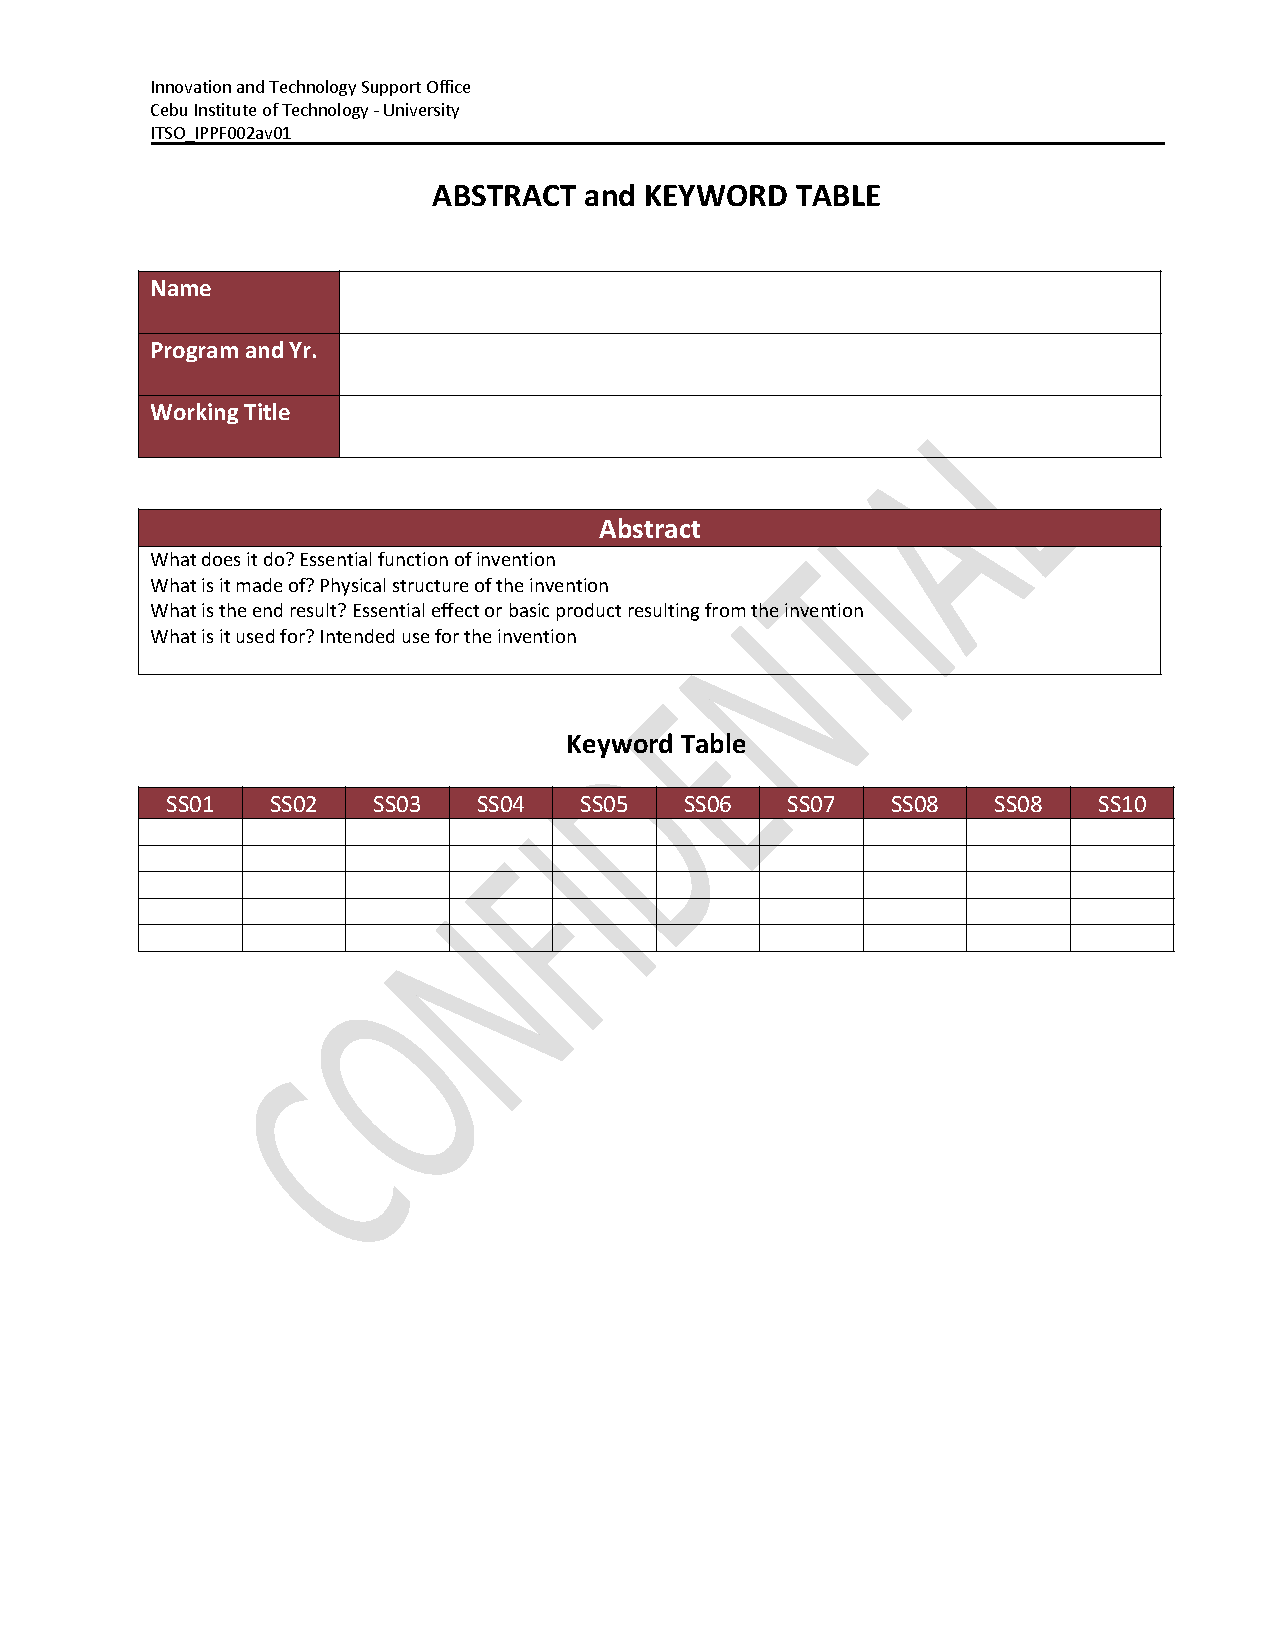
\includepdf[pages=-]{App_AbstractKeyword_member2.pdf}
%XXXXXXXX\includepdf[pages=-]{App_AbstractKeyword_member3.pdf}
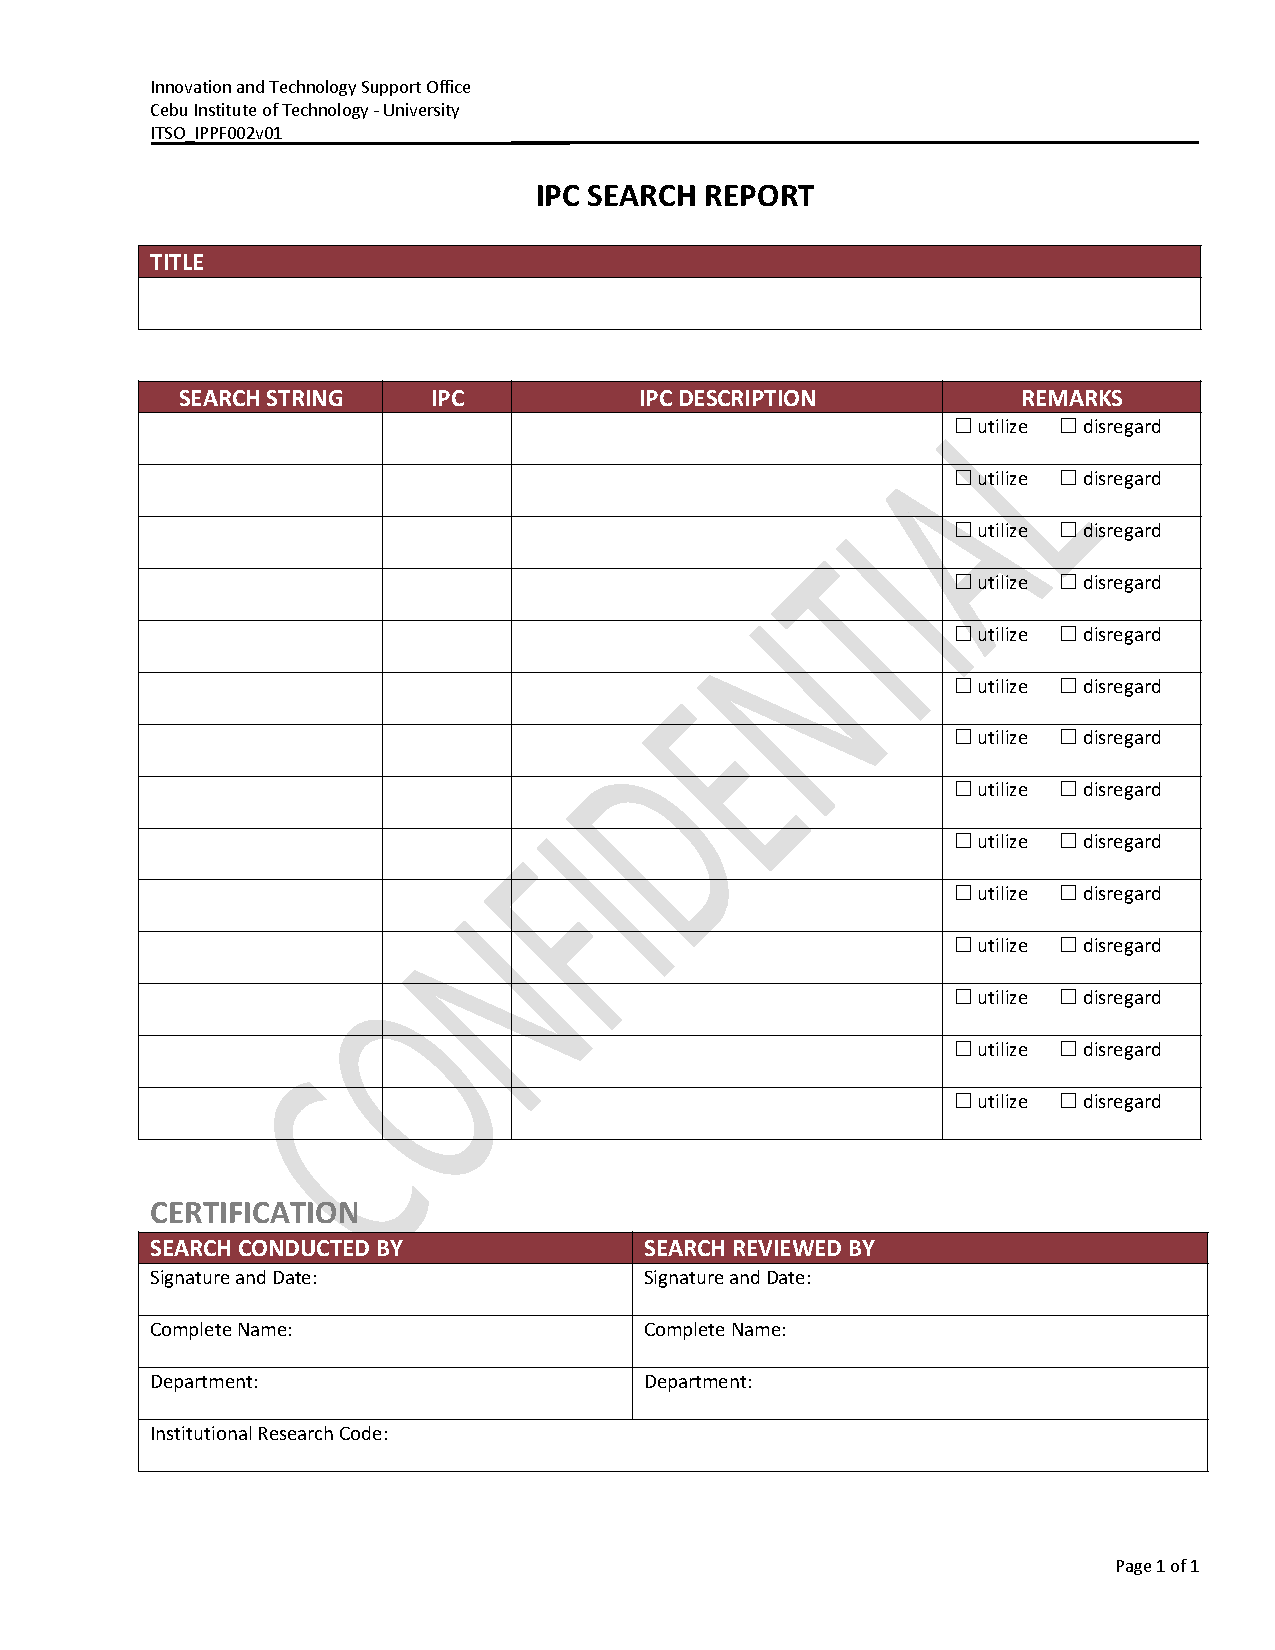
\includepdf[pages=-]{App_ISR_member1.pdf}
%XXXXXXXX\includepdf[pages=-]{App_ISR_member2.pdf}
%XXXXXXXX\includepdf[pages=-]{App_ISR_member3.pdf}
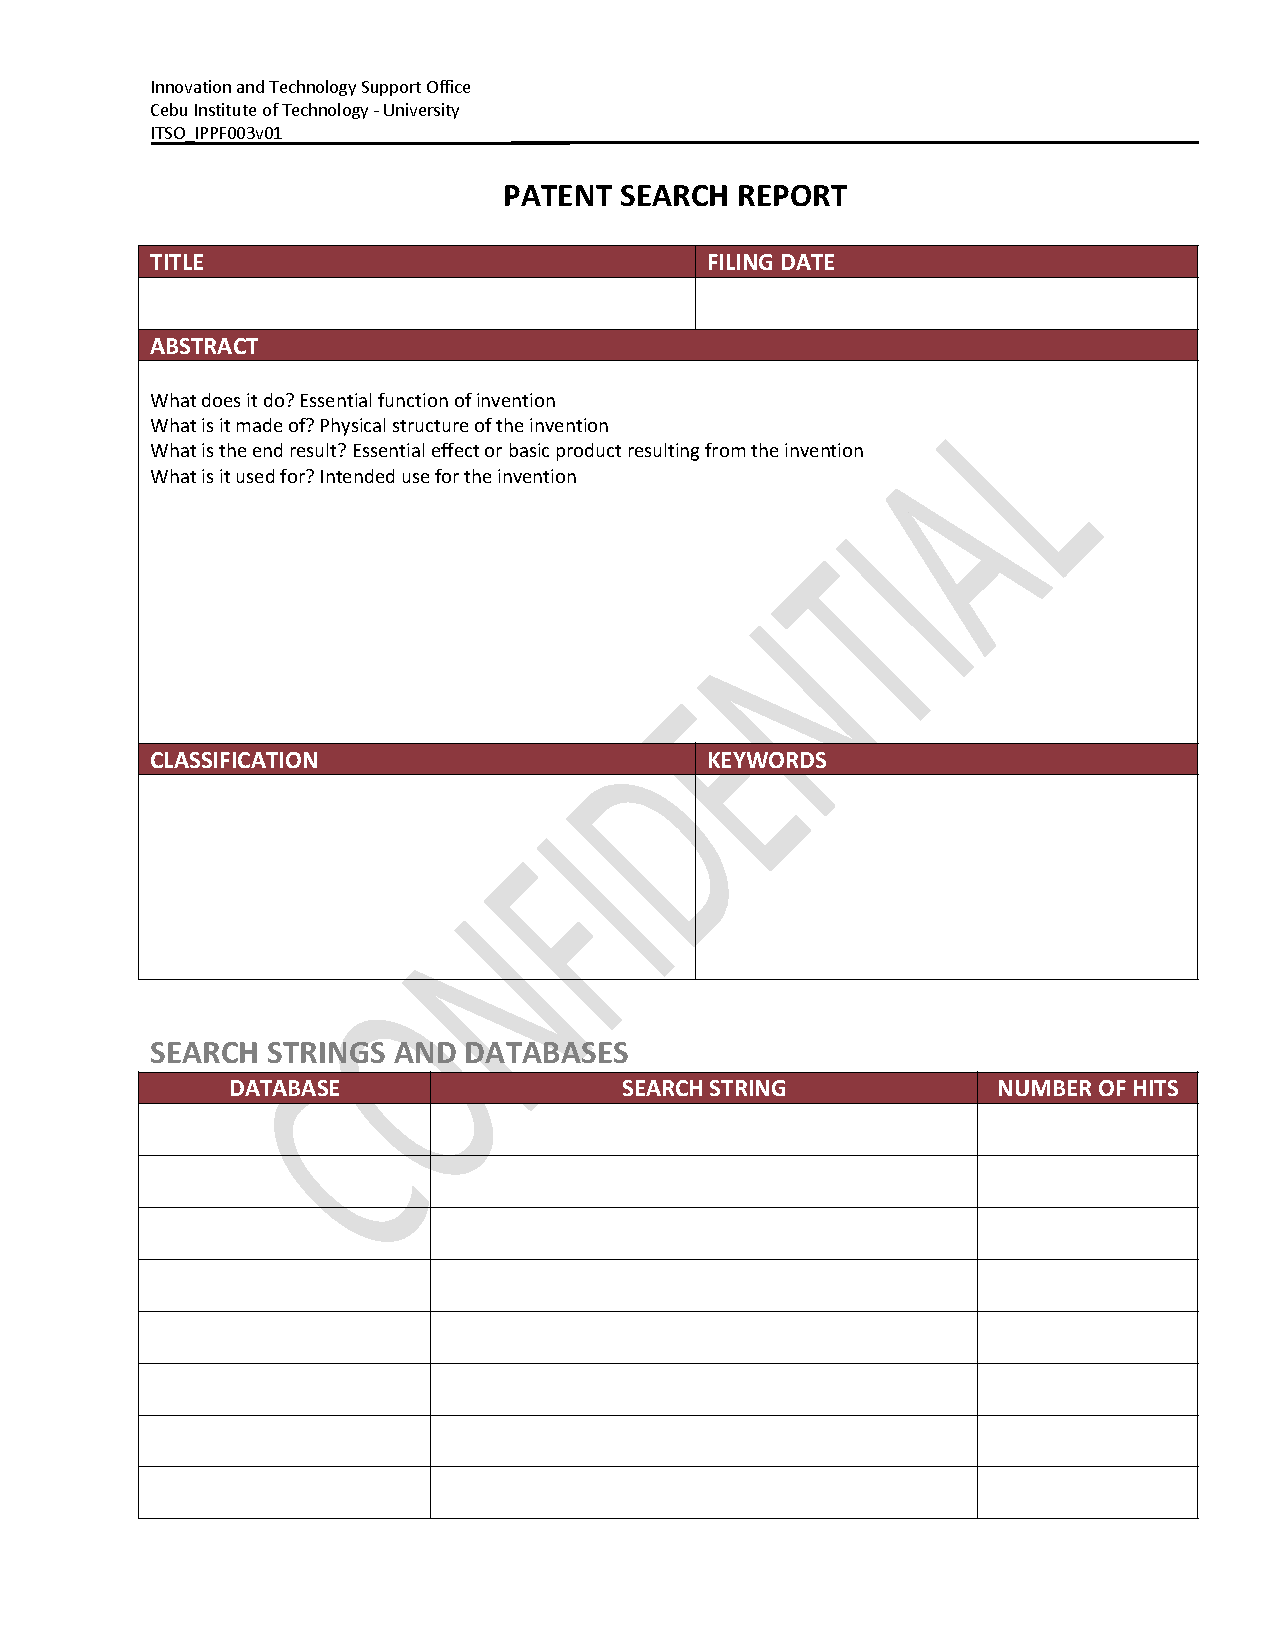
\includepdf[pages=-]{App_PASAR_member1.pdf}
%XXXXXXXX\includepdf[pages=-]{App_PASAR_member2.pdf}
%XXXXXXXX\includepdf[pages=-]{App_PASAR_member3.pdf}
%==========================================================
%XXXXXXXX\newpage
%XXXXXXXX\appendix
%XXXXXXXX\renewcommand{\chaptername}{\appendixname}
%XXXXXXXX\addtocontents{toc}{\protect\renewcommand\protect\chaptername{\appendixname}}
%XXXXXXXX\chapter{PATENT ANALYTICS REPORT}
%-----> REQUIRED IN PROJECT 1
%-----> MUST BE UPDATED IN 2
%XXXXXXXX\includepdf[pages=-]{App_GroupName_PAR.pdf}
%==========================================================
\newpage
\appendix
\renewcommand{\chaptername}{\appendixname}
\addtocontents{toc}{\protect\renewcommand\protect\chaptername{\appendixname}}
\chapter{PATENT DRAFT}
%-----> REQUIRED IN PROJECT 2
%-----> Based on your output in the Workshop on Patent Drafting, print the docx file to pdf then insert it here.
%-----> Only ONE SET of files is required per group
%-----> Use the official template from ITSO
%use includegraphics for the 1st page of the 1st document only
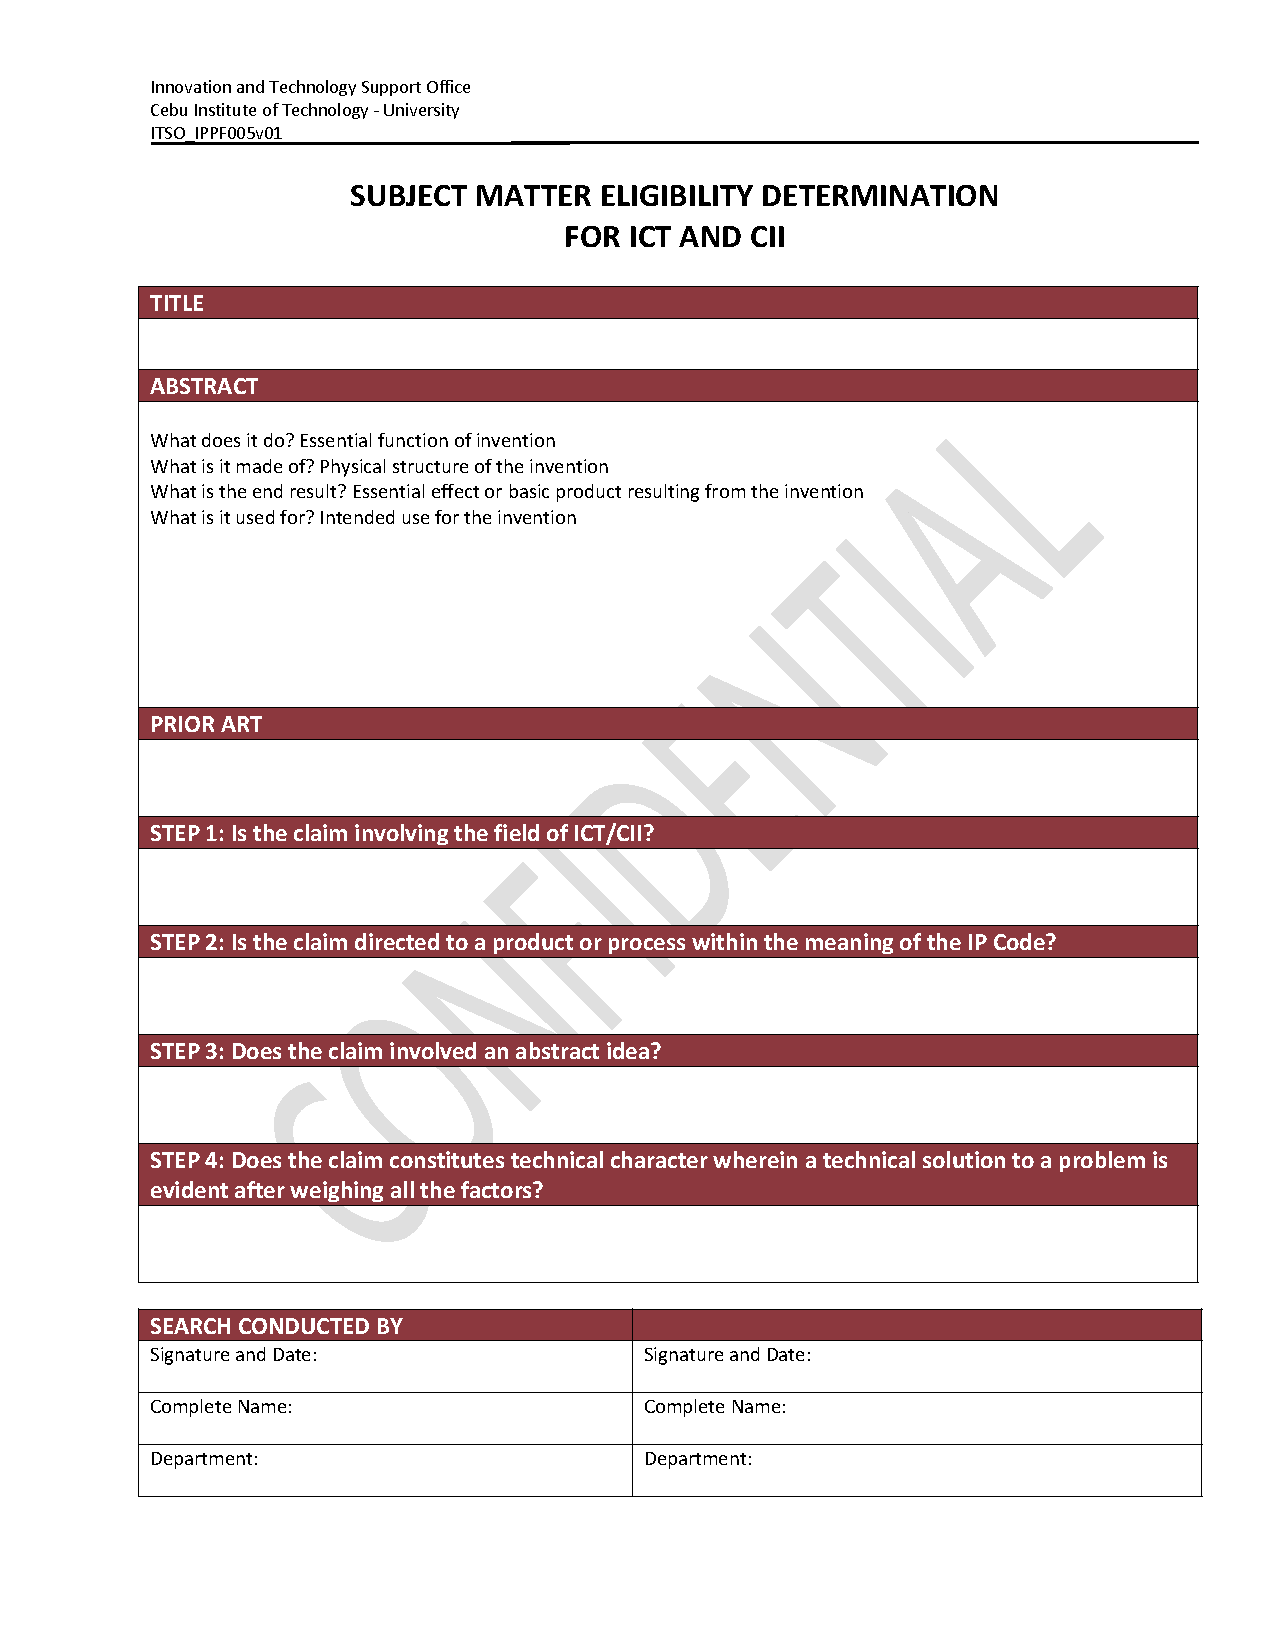
\includegraphics[page=1,width=\textwidth]{App_GroupName_PD_IPPF005v01.pdf}
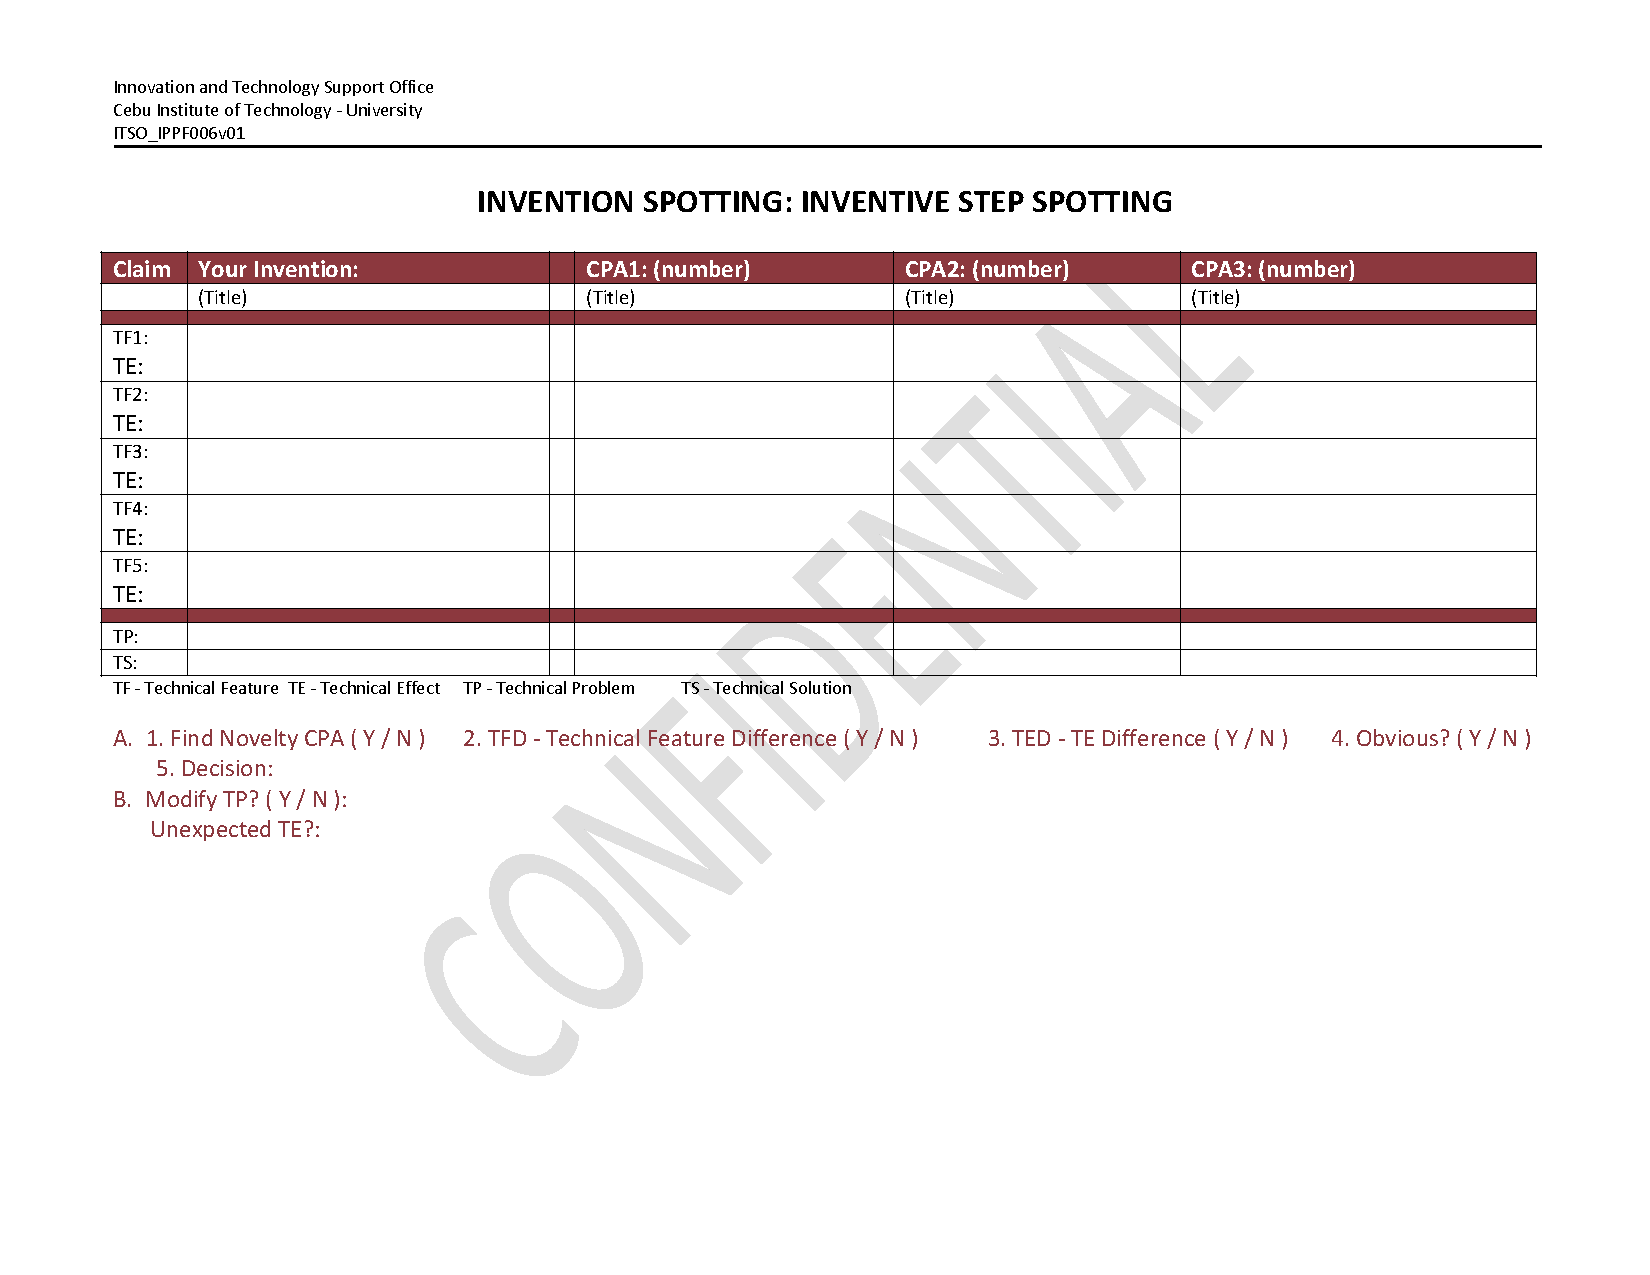
\includepdf[pages=-]{App_GroupName_PD_IPPF006v01.pdf}

\includepdf[pages=-]{App_GroupName_PD_IPPF007v01.pdf}
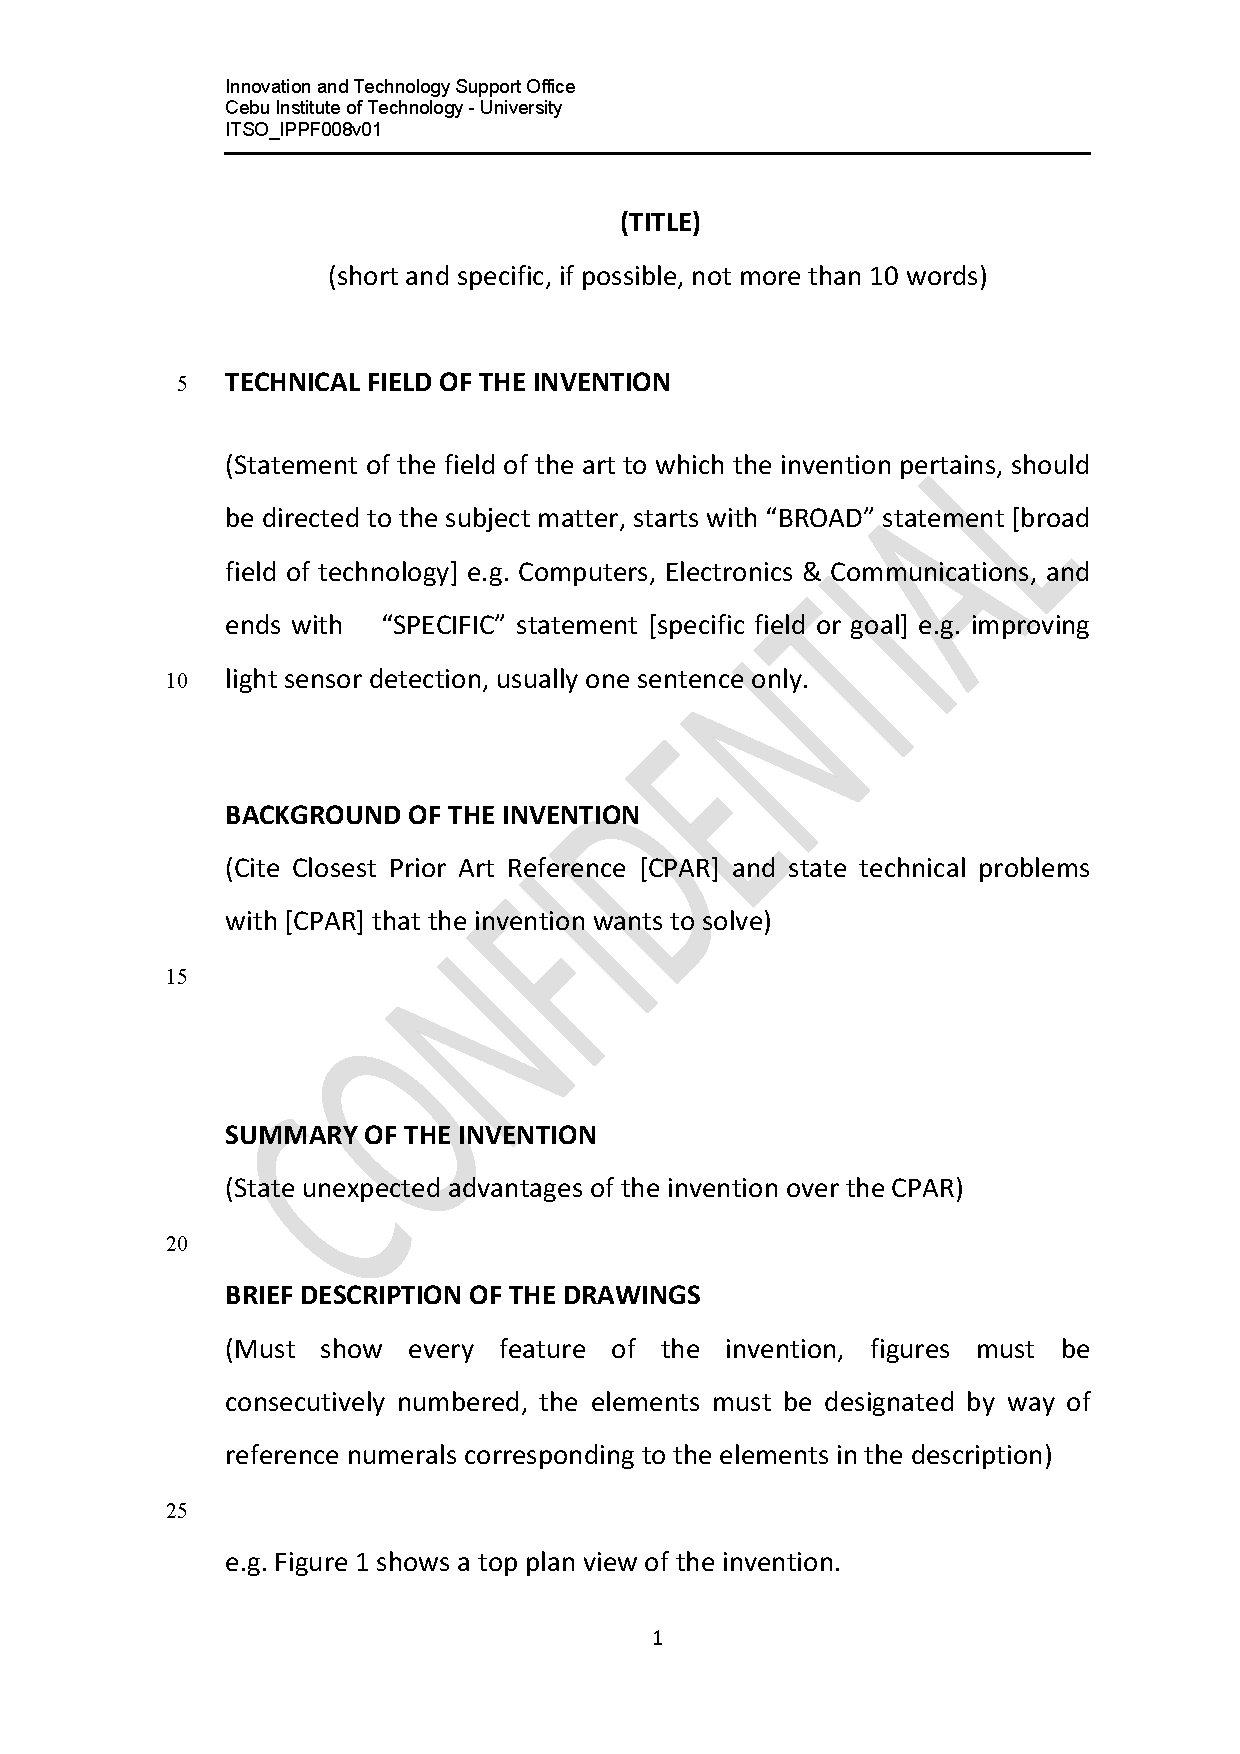
\includepdf[pages=-]{App_GroupName_PD_IPPF008v01.pdf}

%----------------------------------------------------------
%XXXXXXXX\newpage
%XXXXXXXX\chapter{ADVISER'S ACCEPTANCE}
%-----> REQUIRED IN PROJECT 1
%-----> MUST BE UPDATED IN PROJECT 2
%XXXXXXXXInsert the scanned copy of the adviser's acceptance.
This is a figure with NO number and caption.
%----------------------------------------------------------
\newpage
\chapter{TIMETABLE OF ACTIVITIES}
%-----> REQUIRED INPROJECT 1
%-----> MUST BE UPDATED IN PROJECT 1 and 2
%-----> Choose only one type of Gantt chart.
%##############################################################################
%>> two charts for the whole year
%==========================================================
\begin{center}
%==========================================================
\begin{ganttchart}[
%>> height of the title
y unit title=0.4cm,
%>> specify the height of the chart lines
y unit chart=0.5cm, 
%>> show the horizontal grids with the default style
hgrid, 
%>> show the vertical grids with the default style
vgrid,
%>> vertical position of the title label
title label anchor/.style={below=-1.3ex}, 
%>> shift the coordinates of a title element's borders or corners
title left shift=.05,
title right shift=-.05,
%>> height of the title
title height=1,
%>> color of the bars (USE SHADES OF GRAY ONLY)
bar/.style={fill=gray!50},
%>> color of the bar in progress
incomplete/.style={fill=white},
%>> label of a bar in progress
progress label text={},
%>> height of the progress bar
bar height=0.7,
%>> shift the coordinates of a group's borders or corners
group right shift=0,
group top shift=.6,
%>> height of the group
group height=.3,
%>> dimension of the left and right peaks
%group peaks={}{}{.2}
]{1}{24}
%========> TITLE/COLUMN HEADERS AND NUMBER OF COLUMNS
% do not change this part
\gantttitle{Month, S.Y. 2016 -- 2017}{24} \\ 
\gantttitle{Apr}{4} %(one column = one week)
\gantttitle{May}{4} 
\gantttitle{Jun}{4} 
\gantttitle{Jul}{4} 
\gantttitle{Aug}{4} 
\gantttitle{Sept}{4}
%========> TASKS AND COLUMNS BEING OCCUPIED
%****specify the tasks to be done (FOR April to Sept ONLY)*****
%****you can change the number of tasks depending on your project
%****columns  1 to  4: April activities 
%****columns  5 to  8: May activities
%****columns  9 to 12: June activities
%****columns 13 to 16: July activities
%****columns 17 to 20: August activities
%****columns 21 to 24: September activities
%****SYNTAX: \\ \ganttbar{specific task}{starting column}{ending column} 
\\ \ganttbar{task A}{1}{2}    %1st task = elem0 (1st task IN THIS CHART)
\\ \ganttbar{task B}{3}{8}    %2nd task = elem1
\\ \ganttbar{task C}{9}{10}   %3rd task = elem2
\\ \ganttbar{task D}{11}{15}  %4th task = elem3
\\ \ganttbar{task E}{20}{22}  %5th task = elem4 
\\ \ganttbar{task F}{18}{19}  %6th task = elem5 
\\ \ganttbar{task G}{16}{24}  %7th task = elem6 
\\ \ganttbar{task H}{21}{24}  %8th task = elem7
%========> RELATIONSHIPS BETWEEN TASKS
%****specify the relationship between tasks*****
%****the number beside elem depends on the number of tasks
%****refer to the list above (ganttbar)
%****you can change the number of links depending on your project
\ganttlink{elem0}{elem1} 
\ganttlink{elem0}{elem3} 
\ganttlink{elem1}{elem2} 
\ganttlink{elem3}{elem4} 
\ganttlink{elem1}{elem5} 
\ganttlink{elem3}{elem5} 
\ganttlink{elem2}{elem6} 
\ganttlink{elem3}{elem6} 
\ganttlink{elem5}{elem7} 
\end{ganttchart}
%==========================================================
\begin{ganttchart}[
y unit title=0.4cm,
y unit chart=0.5cm,
hgrid, 
vgrid,
title label anchor/.style={below=-1.4ex},
title left shift=.05,
title right shift=-.05,
title height=1,
bar/.style={fill=gray!50},
incomplete/.style={fill=white},
progress label text={},
bar height=0.7,
group right shift=0,
group top shift=.6,
group height=.5,
%group peaks={}{}{.2}
]{1}{24}
%========> TITLE/COLUMN HEADERS AND NUMBER OF COLUMNS
% do not change this part
\gantttitle{Month, S.Y. 2016 -- 2017}{24} \\ 
\gantttitle{Oct}{4} %(one column = one week)
\gantttitle{Nov}{4} 
\gantttitle{Dec}{4} 
\gantttitle{Jan}{4} 
\gantttitle{Feb}{4} 
\gantttitle{Mar}{4} 
%========> TASKS AND COLUMNS BEING OCCUPIED
%****specify the tasks to be done (FOR Oct to March ONLY)*****
%****you can change the number of tasks depending on your project
%****columns  1 to  4: October activities
%****columns  5 to  8: November activities
%****columns  9 to 12: December activities
%****columns 13 to 16: January activities
%****columns 17 to 20: February activities
%****columns 21 to 24: March activities
\\ \ganttbar{task I}{1}{2}    %1st task = elem0 (1st task IN THIS CHART)
\\ \ganttbar{task J}{3}{8}    %2nd task = elem1
\\ \ganttbar{task K}{9}{10}   %3rd task = elem2
\\ \ganttbar{task L}{11}{15}  %4th task = elem3
\\ \ganttbar{task M}{20}{22}  %5th task = elem4
\\ \ganttbar{task N}{18}{19}  %6th task = elem5
\\ \ganttbar{task O}{16}{24}  %7th task = elem6
\\ \ganttbar{task P}{21}{24}  %8th task = elem7
%========> RELATIONSHIPS BETWEEN TASKS
%****specify the relationship between tasks*****
%****the number beside elem depends on the number of tasks
%****refer to the list above (ganttbar)
%****you can change the number of links depending on your project
\ganttlink{elem0}{elem1} 
\ganttlink{elem0}{elem3} 
\ganttlink{elem1}{elem2} 
\ganttlink{elem3}{elem4} 
\ganttlink{elem1}{elem5} 
\ganttlink{elem3}{elem5} 
\ganttlink{elem2}{elem6} 
\ganttlink{elem3}{elem6} 
\ganttlink{elem5}{elem7} 
\end{ganttchart}
%==========================================================
\end{center}

%##############################################################################
%>> one chart for the whole year
%==========================================================
\newpage
\begin{sideways}
\centering
\begin{ganttchart}[
x unit=0.4cm, %width of each column
y unit title=0.4cm,
y unit chart=0.5cm,
hgrid, 
vgrid,
title label anchor/.style={below=-1.4ex},
title left shift=.05,
title right shift=-.05,
title height=1,
bar/.style={fill=gray!50},
incomplete/.style={fill=white},
progress label text={},
bar height=0.7,
group right shift=0,
group top shift=.6,
group height=.5,
%group peaks={}{}{.2}
]{1}{48}
%========> TITLE/COLUMN HEADERS AND NUMBER OF COLUMNS
% do not change this part
\gantttitle{Month, S.Y. 2016 -- 2017}{48} \\ 
\gantttitle{Apr}{4} %(one column = one week)
\gantttitle{May}{4} 
\gantttitle{Jun}{4} 
\gantttitle{Jul}{4} 
\gantttitle{Aug}{4} 
\gantttitle{Sept}{4}
\gantttitle{Oct}{4} 
\gantttitle{Nov}{4} 
\gantttitle{Dec}{4} 
\gantttitle{Jan}{4} 
\gantttitle{Feb}{4} 
\gantttitle{Mar}{4} 
%========> TASKS AND COLUMNS BEING OCCUPIED
%****specify the tasks to be done (FOR Oct to March ONLY)*****
%****you can change the number of tasks depending on your project
%****columns  1 to  4: April activities 
%****columns  5 to  8: May activities
%****columns  9 to 12: June activities
%****columns 13 to 16: July activities
%****columns 17 to 20: August activities
%****columns 21 to 24: September activities
%****columns 25 to 28: October activities
%****columns 29 to 32: November activities
%****columns 33 to 36: December activities
%****columns 37 to 40: January activities
%****columns 41 to 44: February activities
%****columns 45 to 48: March activities
\\ \ganttbar{task A}{1}{2}    % 1st task = elem0 (1st task IN THIS CHART)
\\ \ganttbar{task B}{3}{8}    % 2nd task = elem1
\\ \ganttbar{task C}{9}{10}   % 3rd task = elem2
\\ \ganttbar{task D}{11}{15}  % 4th task = elem3
\\ \ganttbar{task E}{20}{22}  % 5th task = elem4 
\\ \ganttbar{task F}{18}{19}  % 6th task = elem5 
\\ \ganttbar{task G}{16}{24}  % 7th task = elem6 
\\ \ganttbar{task H}{21}{27}  % 8th task = elem7
\\ \ganttbar{task I}{25}{30}  % 9th task = elem8
\\ \ganttbar{task J}{28}{38}  %10th task = elem9
\\ \ganttbar{task K}{37}{40}  %11th task = elem10
\\ \ganttbar{task L}{40}{45}  %12th task = elem11
\\ \ganttbar{task M}{38}{48}  %13th task = elem12
\\ \ganttbar{task N}{28}{44}  %14th task = elem13
\\ \ganttbar{task O}{39}{45}  %15th task = elem14
\\ \ganttbar{task P}{28}{40}  %16th task = elem15
\\ \ganttbar{task P}{37}{42}  %16th task = elem15
\\ \ganttbar{task Q}{25}{41}  %16th task = elem15
\\ \ganttbar{task R}{20}{38}  %16th task = elem15
\\ \ganttbar{task S}{34}{39}  %16th task = elem15
\\ \ganttbar{task T}{23}{48}  %16th task = elem15
\\ \ganttbar{task U}{17}{48}  %16th task = elem15
%========> RELATIONSHIPS BETWEEN TASKS
%****specify the relationship between tasks*****
%****the number beside elem depends on the number of tasks
%****refer to the list above (ganttbar)
%****you can change the number of links depending on your project
\ganttlink{elem0}{elem1} 
\ganttlink{elem0}{elem3} 
\ganttlink{elem1}{elem2} 
\ganttlink{elem3}{elem4} 
\ganttlink{elem1}{elem5} 
\ganttlink{elem3}{elem5} 
\ganttlink{elem2}{elem6} 
\ganttlink{elem3}{elem6} 
\ganttlink{elem5}{elem7} 
\end{ganttchart}
\end{sideways}
%##############################################################################
%>> involvement of each member in the group
%==========================================================
\newpage
\begin{center}
\begin{tabular}{|c|l||c|c|c|c|}
\hline
Task & Task Description & FamilyN1 & FamilyN2 & FamilyN3 & FamilyN4\\
\hline
\hline
A & Specific activity & \cellcolor{gray!50} & \cellcolor{gray!50} &  & \\ \hline
B & Specific activity & \cellcolor{gray!50} &  & \cellcolor{gray!50} & \cellcolor{gray!50}\\ \hline
C & Specific activity &  & \cellcolor{gray!50} &  & \\ \hline
D & Specific activity &  &  & \cellcolor{gray!50} & \\ \hline
E & Specific activity &  &  &  & \cellcolor{gray!50}\\ \hline
F & Specific activity & \cellcolor{gray!50} &  &  & \\ \hline
G & Specific activity &  & \cellcolor{gray!50} &  & \\ \hline
H & Specific activity &  &  & \cellcolor{gray!50} & \\ \hline
I & Specific activity &  &  &  & \cellcolor{gray!50}\\ \hline
J & Specific activity & \cellcolor{gray!50} &  & \cellcolor{gray!50} & \\ \hline
K & Specific activity &  & \cellcolor{gray!50} & \cellcolor{gray!50} & \\ \hline
L & Specific activity &  &  & \cellcolor{gray!50} & \cellcolor{gray!50}\\ \hline
M & Specific activity & \cellcolor{gray!50} & \cellcolor{gray!50} &  & \cellcolor{gray!50}\\ \hline
N & Specific activity &  & \cellcolor{gray!50} &  & \cellcolor{gray!50}\\ \hline
O & Specific activity & \cellcolor{gray!50} &  & \cellcolor{gray!50} & \\ \hline
P & Specific activity & \cellcolor{gray!50} & \cellcolor{gray!50} &  & \\ \hline
Q & Specific activity & \cellcolor{gray!50} & \cellcolor{gray!50} & \cellcolor{gray!50} & \cellcolor{gray!50}\\ \hline
R & Specific activity & \cellcolor{gray!50} &  &  & \cellcolor{gray!50}\\ \hline
S & Specific activity &  &  & \cellcolor{gray!50} & \cellcolor{gray!50}\\ \hline
T & Specific activity &  & \cellcolor{gray!50} &  & \\ \hline
U & Specific activity &  &  & \cellcolor{gray!50} & \\ \hline
\end{tabular}
\end{center}

%----------------------------------------------------------
\newpage
\chapter{RESEARCH BUDGET}
%-----> REQUIRED INPROJECT 1
%-----> MUST BE UPDATED IN PROJECT 1 and 2
This is the budget of the thesis or project.
During proposal, tabulate the possible expenses here.
You can use a \textbf{long table} if your list of expenses spans several pages.
In order to prevent your tables from floating, use the \textbf{tabular} environment only.
List of expenses can be shorter by grouping them according to semester or a certain span of time.
Item description and quantity should be left justified and centered, respectively.
Amount should be right justified with two decimal places and comma for those that reach or exceed 1,000.00.

%----------------------------------------------------------
\newpage
\chapter{ADDITIONAL FLOWCHARTS}
%-----> IF APPLICABLE
%-----> MUST BE UPDATED IN PROJECT 1 and 2
This appendix is for supplemental flowcharts only.
Those that are for the main program or system should be inside Chapter~\ref{chap:method}.
Figures here should also be cross-referenced or mentioned in other chapters.
%----------------------------------------------------------
\newpage
\chapter{PSEUDO-CODES}
%-----> IF APPLICABLE
%-----> MUST BE UPDATED IN PROJECT 1 and 2
Insert pseudo-code of your algorithms here. 
Use the \texttt{algorithmic} environment. 
Below is an example:

\begin{algorithm}
\caption{Euclid's algorithm}
\label{algo: euclid}
\begin{algorithmic}[1]
\Procedure{Euclid}{$a,b$}\Comment{The g.c.d. of a and b}
\State $r\gets a\bmod b$
\While{$r\not=0$}\Comment{We have the answer if r is 0}
\State $a\gets b$
\State $b\gets r$
\State $r\gets a\bmod b$
\EndWhile\label{euclidendwhile}
\State \textbf{return} $b$\Comment{The gcd is b}
\EndProcedure
\end{algorithmic}
\end{algorithm}

If additional programs used in the experiment will be inserted, CHANGE the chapter title in the main tex file (line 173) to \text{Experiment Codes}.
First, indicate the name of the program/code with file extension (ex. test1.sci) then enclose the commands with the \text{verbatim} environment.
%----------------------------------------------------------
\newpage
\chapter{ELECTRICAL CIRCUITS}
%-----> IF APPLICABLE
%-----> MUST BE UPDATED IN PROJECT 1 and 2
Insert supplemental circuit diagrams here.
Examples are power supply circuits (customized for the prototype) and driver circuits (not part of the main methodology).
Insert the diagram as \textbf{figure} and cross-reference or mention these in other chapters.

%----------------------------------------------------------
\newpage
\chapter{SUPPLEMENTAL DATA}
%-----> IF APPLICABLE
%-----> MUST BE UPDATED IN PROJECT 1 and 2
Insert your raw data here in tabular form (data from 100 trials).
The tables MUST HAVE numbers and captions, i.e. use the \textbf{table} environment.
If applicable, use long table with headers and footers.
You can also cross-reference the tables here in your discussions in other chapters.
Note that the data here should be summarized in a separate table or graph that is placed in Chapter~\ref{chap:results}.

%----------------------------------------------------------
\newpage
\chapter{PLAGIARISM CHECK REPORT}
%-----> REQUIRED IN PROJECT 2
%-----> This should be the Turnitin report for the FINAL VERSION of your document, the version after final defense and approved by the advoiser and panelists.
%-----> In submitting to Turnitin, the title of your submission should be: Groupname-Abstract, Groupname-Chapter 1, Groupname-Chapter 2, Groupname-Chapter 3, Groupname-Chapter 4, Groupname-Chapter 5 
%Insert the scanned copy of the results from Turnitin.
%The figures must have NO number and caption.
%ALL PAGES must be inserted here.
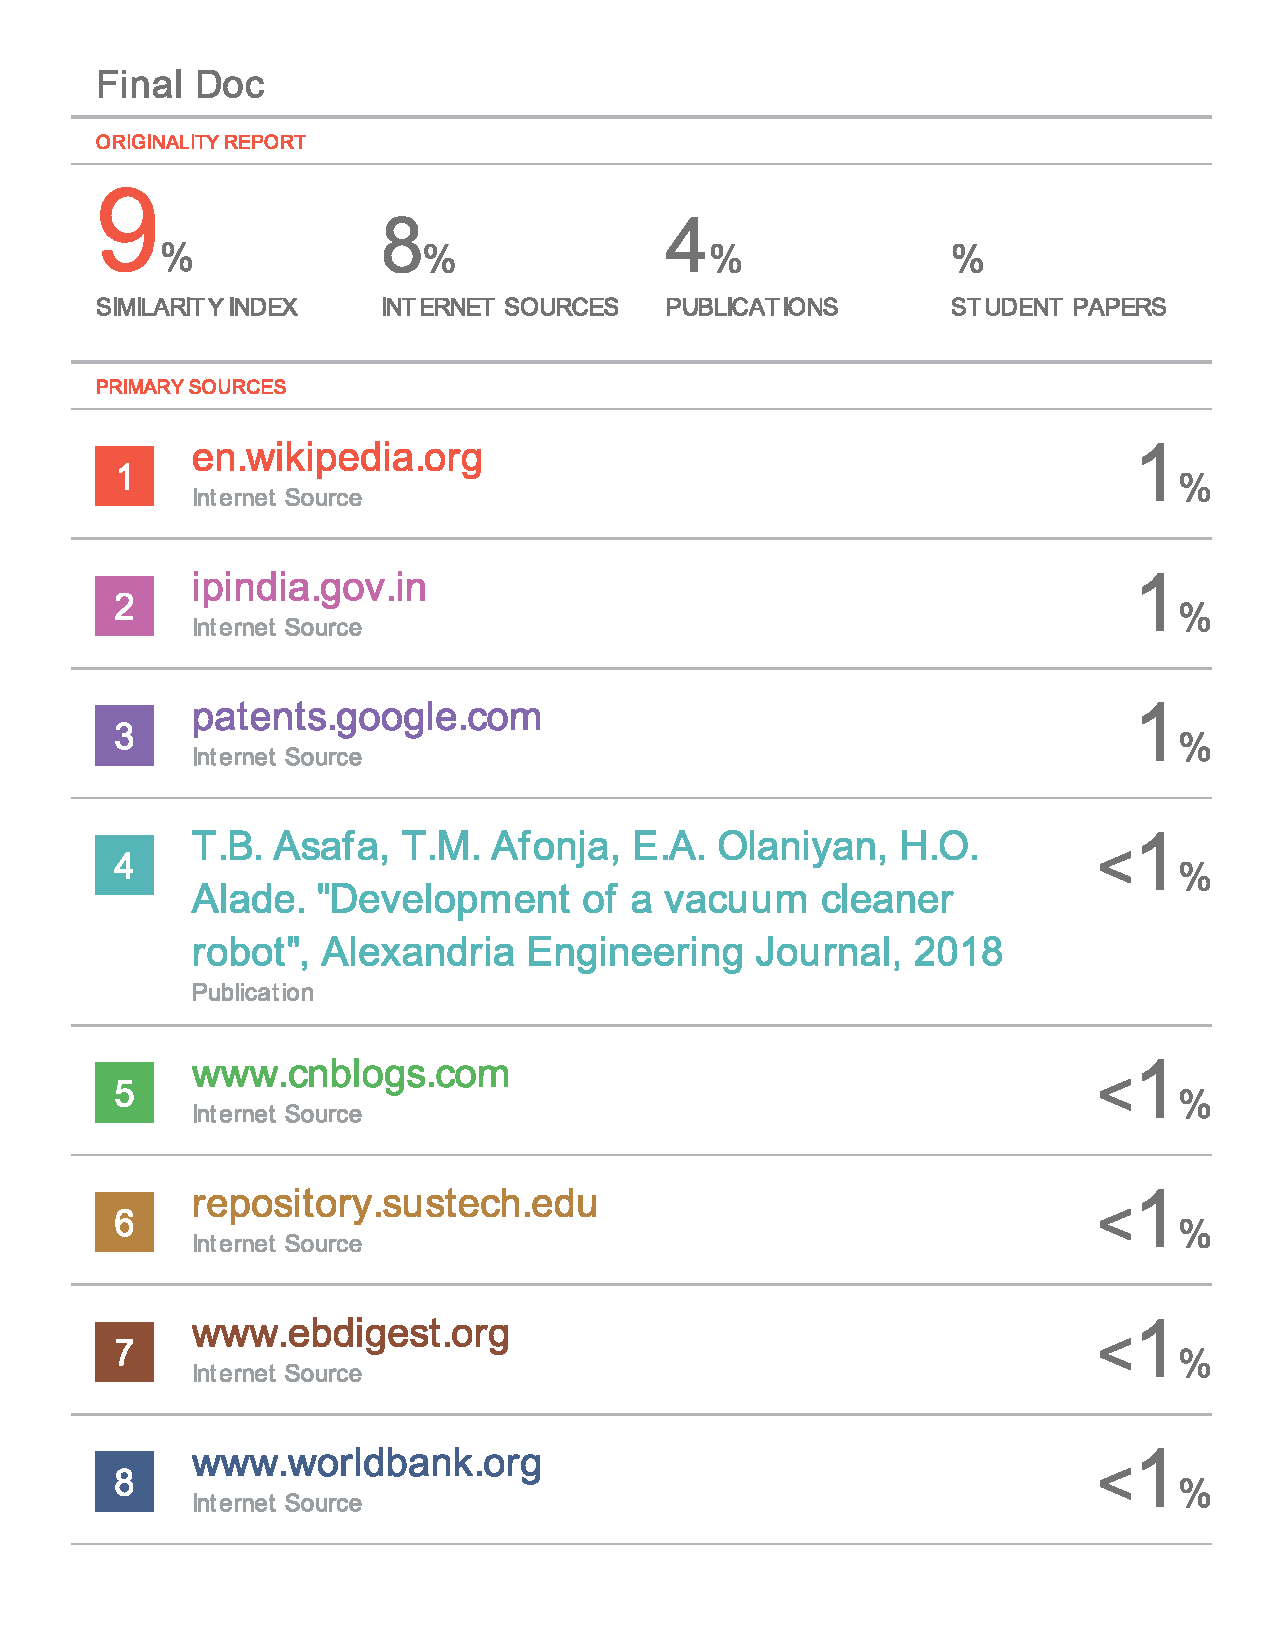
\includegraphics[page=1,width=\textwidth]{Turnitin_sample_abstract.pdf}
\newpage 
\includegraphics[page=2,width=\textwidth]{Turnitin_sample_abstract.pdf}
\newpage 
\includegraphics[page=3,width=\textwidth]{Turnitin_sample_abstract.pdf}
\newpage 
\includegraphics[page=4,width=\textwidth]{Turnitin_sample_abstract.pdf}
\newpage 
\includegraphics[page=5,width=\textwidth]{Turnitin_sample_abstract.pdf}
\newpage 
\includegraphics[page=6,width=\textwidth]{Turnitin_sample_abstract.pdf}
\newpage 
\includegraphics[page=7,width=\textwidth]{Turnitin_sample_abstract.pdf}
\newpage 
\includegraphics[page=8,width=\textwidth]{Turnitin_sample_abstract.pdf}
%\newpage
%\includegraphics[page=1,width=\textwidth]{Turnitin_sample_chap1.pdf}
%\newpage
%\includegraphics[page=1,width=\textwidth]{Turnitin_sample_chap2.pdf}
%\newpage
%\includegraphics[page=1,width=\textwidth]{Turnitin_sample_chap3.pdf}
%\newpage
%\includegraphics[page=1,width=\textwidth]{Turnitin_sample_chap4.pdf}
%\newpage
%\includegraphics[page=1,width=\textwidth]{Turnitin_sample_chap5.pdf}
%----------------------------------------------------------
\newpage
\chapter{ETHICS CLEARANCE}
%-----> REQUIRED IN PROJECT 2
%-----> This should be obtained right after the proposal hearing, once your topic is already approved.

\includegraphics[page=1,width=\textwidth]{App_EthicsClearance.pdf}
\newpage 

\includegraphics[page=2,width=\textwidth]{App_EthicsClearance.pdf}

%----------------------------------------------------------
\newpage
\chapter{CURRICULUM VITAE}
%-----> REQUIRED IN PROJECT 2
%-----> this should be the LAST CHAPTER
%-----> if possible, insert your grad picture
%-----> if you do not have any entry on any item, remove them and DO NOT PUT NONE
%\begin{wrapfigure}{r}{2in}%{0.5 \textwidth}
%\vspace{-20pt}
%\begin{flushright}
%
\includegraphics[width=1in,height=1in]{cea_seal}
%\end{flushright}
%\vspace{-20pt}
%\end{wrapfigure}
\begin{figure*}[h]
\vspace{-20pt}
\begin{flushright}

\includegraphics[width=1in,height=1in]{cea_seal.jpg}
\end{flushright}
\vspace{-30pt}
\end{figure*}
{\singlespace
\noindent \underline{CONTACT INFORMATION}
\begin{itemize}
\item[] \textbf{Name:} Given Name MI. Family Name
\item[] \textbf{Address:} Number and Street, City or Province, Philippines, Zip Code
\item[] \textbf{Telephone Number:} 063 - area code - number
\item[] \textbf{Cell Phone Number:} 09numbers
\item[] \textbf{Email:} address@site.dmn
\end{itemize}
}

{\singlespace
\noindent \underline{PERSONAL INFORMATION}
\begin{itemize}
\item[] \textbf{Date of Birth:} Month DD, YYYY\\
\textbf{Place of Birth:} City, Country\\
\textbf{Citizenship:} Filipino
\end{itemize}
}

{\singlespace
\noindent \underline{EDUCATIONAL BACKGROUND}
\begin{itemize}
\item[] \textbf{College}\\
Cebu Institute of Technology University\\
N. Bacalso Avenue, Cebu City, Philippines\\
Bachelor of Science in Electronics Engineering\\
March 2013
\item[] \textbf{High School}\\
Name of High School attended\\
Address\\
Month YYYY
\end{itemize}
}

{\singlespace
\noindent \underline{WORK EXPERIENCE} %(if applicable)
\begin{itemize}
\item[] \textbf{Name of Company (latest)}\\
Address\\
Position\\
Responsibilities\\
Inclusive Dates
\item[] \textbf{Name of Company}\\
Address\\
Position\\
Responsibilities\\
Inclusive Dates
\end{itemize}
}

{\singlespace
\noindent \underline{PROFESSIONAL QUALIFICATIONS}
\begin{itemize}
\item[] \textbf{Certifications}\\
certification 1 (latest)\\
certification 2
\item[] \textbf{Computer Skills}\\
skill 1 \\
skill 2
\end{itemize}
}


{\singlespace
\noindent \underline{HONORS AND AWARDS}
\begin{itemize}
\item[] \textbf{Name of Award 1 (latest)}\\
Institution\\
Month, YYYY
\item[] \textbf{Name of Award 2}\\
Institution\\
Month, YYYY
\end{itemize}
}

{\singlespace
\noindent \underline{PROFESSIONAL AFFILIATION}
\begin{itemize}
\item[] \textbf{Name of Organization 1 (latest)}\\
Position\\
Inclusive Years
\item[] \textbf{Name of Organization 2}\\
Position\\
Inclusive Years
\end{itemize}
}

{\singlespace
\noindent \underline{SKILLS AND INTERESTS}
\begin{itemize}
\item[] \textbf{Skills:} skill 1, skill 2, skill 3 
\item[] \textbf{Software:} software 1, software 2, software 3, software 4, software 5
\item[] \textbf{Community Extension:} extension 1, extension 2
\item[] \textbf{Languages:} Language 1 - Native, Language 2 - Fluent, Language 3 - Advanced or Intermediate or Beginner
\end{itemize}
}
\newpage
%\begin{wrapfigure}{r}{2in}%{0.5 \textwidth}
%\vspace{-20pt}
%\begin{flushright}
%
\includegraphics[width=1in,height=1in]{cea_seal.jpg}
%\end{flushright}
%\vspace{-20pt}
%\end{wrapfigure}
\begin{figure*}[h]
\vspace{-20pt}
\begin{flushright}

\includegraphics[width=1in,height=1in]{ecelogo}
\end{flushright}
\vspace{-30pt}
\end{figure*}
{\singlespace
\noindent \underline{CONTACT INFORMATION}
\begin{itemize}
\item[] \textbf{Name:} Given Name MI. Family Name
\item[] \textbf{Address:} Number and Street, City or Province, Philippines, Zip Code
\item[] \textbf{Telephone Number:} 063 - area code - number
\item[] \textbf{Cell Phone Number:} 09numbers
\item[] \textbf{Email:} address@site.dmn
\end{itemize}
}

{\singlespace
\noindent \underline{PERSONAL INFORMATION}
\begin{itemize}
\item[] \textbf{Date of Birth:} Month DD, YYYY\\
\textbf{Place of Birth:} City, Country\\
\textbf{Citizenship:} Filipino
\end{itemize}
}

{\singlespace
\noindent \underline{EDUCATIONAL BACKGROUND}
\begin{itemize}
\item[] \textbf{College}\\
Cebu Institute of Technology University\\
N. Bacalso Avenue, Cebu City, Philippines\\
Bachelor of Science in Electronics Engineering\\
March 2013
\item[] \textbf{High School}\\
Name of High School attended\\
Address\\
Month YYYY
\end{itemize}
}

{\singlespace
\noindent \underline{WORK EXPERIENCE} %(if applicable)
\begin{itemize}
\item[] \textbf{Name of Company (latest)}\\
Address\\
Position\\
Responsibilities\\
Inclusive Dates
\item[] \textbf{Name of Company}\\
Address\\
Position\\
Responsibilities\\
Inclusive Dates
\end{itemize}
}

{\singlespace
\noindent \underline{PROFESSIONAL QUALIFICATIONS}
\begin{itemize}
\item[] \textbf{Certifications}\\
certification 1 (latest)\\
certification 2
\item[] \textbf{Computer Skills}\\
skill 1 \\
skill 2
\end{itemize}
}


{\singlespace
\noindent \underline{HONORS AND AWARDS}
\begin{itemize}
\item[] \textbf{Name of Award 1 (latest)}\\
Institution\\
Month, YYYY
\item[] \textbf{Name of Award 2}\\
Institution\\
Month, YYYY
\end{itemize}
}

{\singlespace
\noindent \underline{PROFESSIONAL AFFILIATION}
\begin{itemize}
\item[] \textbf{Name of Organization 1 (latest)}\\
Position\\
Inclusive Years
\item[] \textbf{Name of Organization 2}\\
Position\\
Inclusive Years
\end{itemize}
}

{\singlespace
\noindent \underline{SKILLS AND INTERESTS}
\begin{itemize}
\item[] \textbf{Skills:} skill 1, skill 2, skill 3 
\item[] \textbf{Software:} software 1, software 2, software 3, software 4, software 5
\item[] \textbf{Community Extension:} extension 1, extension 2
\item[] \textbf{Languages:} Language 1 - Native, Language 2 - Fluent, Language 3 - Advanced or Intermediate or Beginner
\end{itemize}
}
%----------------------------------------------------------
%==========================================================
\end{document}